% Этот текст можно свободно редактировать.
\FloatBarrier
\section{RL: функция цели и обновление}

Используется on-policy grouped REINFORCE с baseline из трёх других траекторий того же реального префикса. На update выбираются 16 train states, по 4 траектории, по 5 действий. Полный softmax по словарю, temperature 1, gamma .9, AdamW lr .0001, 300 updates, clip norm 1. Для каждого RL run сэмплируются 96 000 действий.

На шаге \(t\) используется shaped reward с замороженной reference-политикой SFT:
\begin{align}
\widetilde r_t^{(k)} &= r_t^{(k)}-\beta\log
 \frac{\pi_\theta(a_t^{(k)}\mid s_t^{(k)})}{\pi_{\mathrm{SFT}}(a_t^{(k)}\mid s_t^{(k)})},\\
G_t^{(k)} &= \sum_{j=t}^{H-1}\gamma^{j-t}\widetilde r_j^{(k)},\\
A_t^{(k)} &= G_t^{(k)}-\frac{1}{K-1}\sum_{\ell\ne k}G_t^{(\ell)},
\qquad K=4,\quad H=5.
\end{align}
Остальные три независимо сэмплированные траектории того же начального префикса
задают leave-one-out baseline. Функция потерь имеет вид
\begin{equation}
\mathcal L_{\mathrm{RL}}(\theta)=
-\frac{\mathbb E_k\!\left[\sum_{t=0}^{H-1}\gamma^t\,
 \operatorname{stopgrad}(A_t^{(k)})\log\pi_\theta(a_t^{(k)}\mid s_t^{(k)})\right]}
 {\sum_{t=0}^{H-1}\gamma^t}.
\end{equation}
Усреднение также выполняется по начальным префиксам batch. Sampling и gradient replay
используют одну текущую политику без dropout; после update rollout больше не используется.
При continued-CE dropout также выключен, gradient update остаётся включённым.

При append выбранный ID добавляется в контекст как предположение surrogate среды. В frozen bandit состояние не меняется, а baseline строится по немедленным rewards, поскольку действия не имеют будущих последствий. Это matched по числу actions/updates контроль контекстных переходов, а не ещё одна реалистичная модель пользователя.

Completion сравнивается при \(\beta\in\{0,0.05,0.20\}\). Для других целей:
\begin{align}
r_{\mathrm{seconds}} &= \frac{\min(d,600)\,c}{300},\\
r_{\mathrm{balanced}} &= 0.7c+0.2q+0.1n-0.25I_{\mathrm{recent}}-0.1\sigma_{\mathrm{RM}},\\
n &= 1-\frac{\log(1+\mathrm{train\_count})}{\log(1+\mathrm{max\_count})}.
\end{align}
Здесь \(c\) --- predicted completion, \(q\) --- return proxy, \(d\) --- длительность
трека в секундах, \(n\) --- novelty, \(I_{\mathrm{recent}}\) --- повтор в последних
64 токенах, а \(\sigma_{\mathrm{RM}}\) --- расхождение bootstrap reward models.
Для balanced добавлен \(0.05\mathcal L_{\mathrm{CE}}\) по реальным целям.
Коэффициенты заданы до RL и не подбирались по test.

Checkpoints 100/200/300: максимум собственной ожидаемой validation utility. Balanced сначала требует \ensuremath{\geq}95\% SFT validation NDCG, иначе берёт лучший NDCG и отмечает провал ограничения. Continued-CE выбирается по validation NDCG. Ожидаемые rewards оцениваются 32 Monte Carlo действиями на запрос с общими uniforms для всех политик; ranking считается точно.

Frozen SFT задаёт KL reference, а RM и embeddings не обновляются во время RL. У всех вариантов идентичный каталог и исходные checkpoints. В конфигурации сохранены seeds, horizons, коэффициенты и правило выбора.

\FloatBarrier
\begingroup
\setlength{\tabcolsep}{3pt}
\setlength{\reporttablewidth}{\dimexpr\linewidth-18pt\relax}
\renewcommand{\arraystretch}{1.15}
\small
\begin{longtable}{@{}>{\raggedright\arraybackslash}p{0.23349\reporttablewidth}>{\raggedright\arraybackslash}p{0.30718\reporttablewidth}>{\raggedright\arraybackslash}p{0.22967\reporttablewidth}>{\raggedright\arraybackslash}p{0.22967\reporttablewidth}@{}}
\caption{RL: функция цели и обновление}\label{tab:results-3}\\
\toprule
\textbf{Вариант} & \textbf{Шаги seed 42/43/44} & \textbf{Validation NDCG} & \textbf{SFT floor} \\
\midrule
\endfirsthead
\multicolumn{4}{l}{\small\itshape Продолжение таблицы \thetable}\\
\toprule
\textbf{Вариант} & \textbf{Шаги seed 42/43/44} & \textbf{Validation NDCG} & \textbf{SFT floor} \\
\midrule
\endhead
\midrule
\multicolumn{4}{r}{\footnotesize Продолжение на следующей странице}\\
\endfoot
\bottomrule
\endlastfoot
Continued CE & 100 / 200 / 100 & 0.01479 & не задан \\
Completion, \ensuremath{\beta}=0 & 300 / 300 / 300 & 0.00025 & не задан \\
Completion, \ensuremath{\beta}=.05 & 300 / 300 / 300 & 0.01026 & не задан \\
Completion, \ensuremath{\beta}=.20 & 300 / 300 / 300 & 0.01325 & не задан \\
Секунды, \ensuremath{\beta}=.10 & 300 / 300 / 300 & 0.01227 & не задан \\
Balanced, \ensuremath{\beta}=.10 & 300 / 300 / 200 & 0.01377 & 3/3 \\
Bandit, \ensuremath{\beta}=.05 & 300 / 300 / 300 & 0.01147 & не задан \\
\end{longtable}
\endgroup

\begin{figure}[!htbp]
\centering
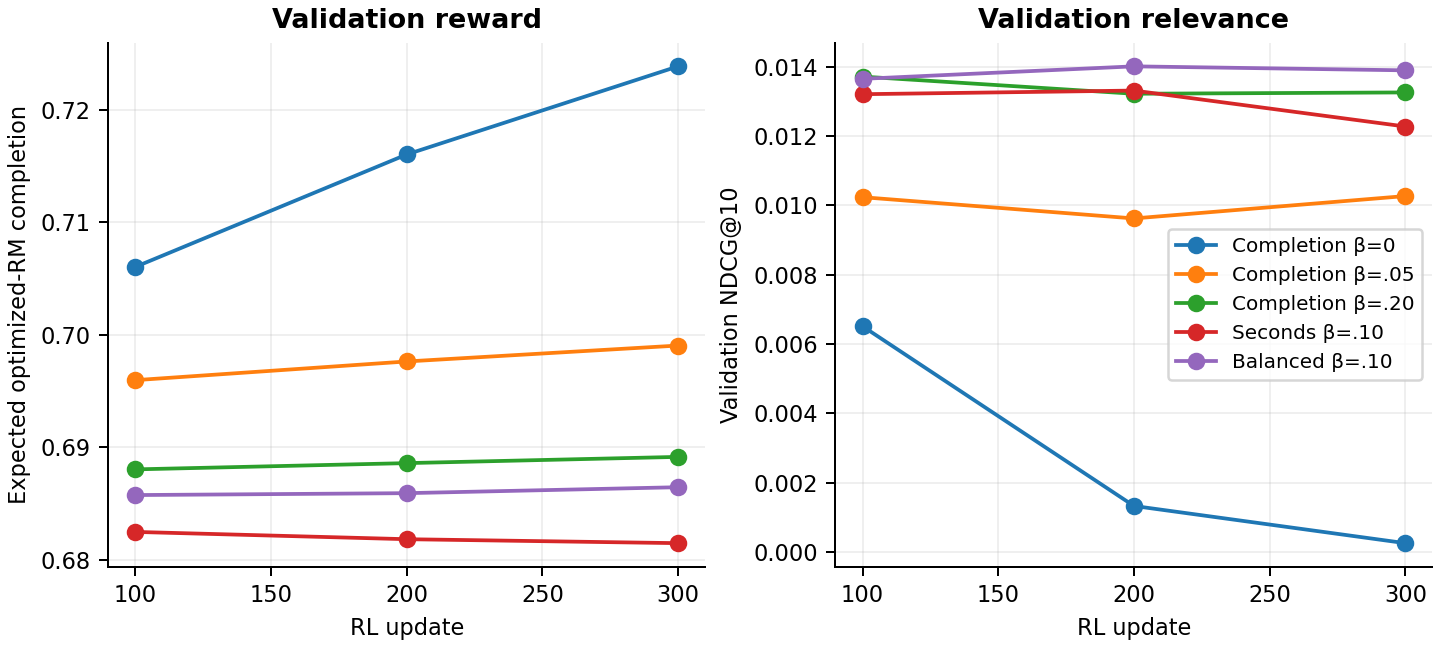
\includegraphics[width=\linewidth,height=.70\textheight,keepaspectratio]{figures/rl_curves.png}
\caption{Validation checkpoints: награда и релевантность могут меняться в разных направлениях. Floor относится только к balanced.}
\label{fig:rl-curves}
\end{figure}
